%%% The main file. It contains definitions of basic parameters and includes all other parts.

%% Settings for single-side (simplex) printing
% Margins: left 40mm, right 25mm, top and bottom 25mm
% (but beware, LaTeX adds 1in implicitly)
\documentclass[12pt,a4paper]{report}
\setlength\textwidth{145mm}
\setlength\textheight{247mm}
\setlength\oddsidemargin{15mm}
\setlength\evensidemargin{15mm}
\setlength\topmargin{0mm}
\setlength\headsep{0mm}
\setlength\headheight{0mm}
% \openright makes the following text appear on a right-hand page
\let\openright=\clearpage

%% Settings for two-sided (duplex) printing
% \documentclass[12pt,a4paper,twoside,openright]{report}
% \setlength\textwidth{145mm}
% \setlength\textheight{247mm}
% \setlength\oddsidemargin{14.2mm}
% \setlength\evensidemargin{0mm}
% \setlength\topmargin{0mm}
% \setlength\headsep{0mm}
% \setlength\headheight{0mm}
% \let\openright=\cleardoublepage



\def\xxx#1{\textbf{\textcolor{red}{xxx: #1}}}
\def\todo#1{\textbf{\textcolor{red}{todo: #1}}}
\def\diff#1{\textbf{\textcolor{green}{#1}}}
\def\equo#1{``#1''}

\def\Tref#1{Table~\ref{#1}}
\def\Fref#1{Figure~\ref{#1}}
\def\Sref#1{Section~\ref{#1}}
\def\footurl#1{\footnote{\url{#1}}}


%% Generate PDF/A-2u
\usepackage[a-2u]{pdfx}

%% Character encoding: usually latin2, cp1250 or utf8:
\usepackage[utf8]{inputenc}

%% Prefer Latin Modern fonts
\usepackage{lmodern}

%% Further useful packages (included in most LaTeX distributions)
\usepackage{amsmath}        % extensions for typesetting of math
\usepackage{amsfonts}       % math fonts
\usepackage{amsthm}         % theorems, definitions, etc.
\usepackage{bbding}         % various symbols (squares, asterisks, scissors, ...)
\usepackage{bm}             % boldface symbols (\bm)
\usepackage{graphicx}       % embedding of pictures
\usepackage{fancyvrb}       % improved verbatim environment
\usepackage{natbib}         % citation style AUTHOR (YEAR), or AUTHOR [NUMBER]
\usepackage[nottoc]{tocbibind} % makes sure that bibliography and the lists
			    % of figures/tables are included in the table
			    % of contents
\usepackage{dcolumn}        % improved alignment of table columns
\usepackage{booktabs}       % improved horizontal lines in tables
\usepackage{paralist}       % improved enumerate and itemize
\usepackage[usenames]{xcolor}  % typesetting in color

\usepackage{multirow}
%%% Basic information on the thesis

% Thesis title in English (exactly as in the formal assignment)
\def\ThesisTitle{Thesis title}

% Author of the thesis
\def\ThesisAuthor{Name Surname}

% Year when the thesis is submitted
\def\YearSubmitted{YEAR}

% Name of the department or institute, where the work was officially assigned
% (according to the Organizational Structure of MFF UK in English,
% or a full name of a department outside MFF)
\def\Department{Name of the department}

% Is it a department (katedra), or an institute (ústav)?
\def\DeptType{Department}

% Thesis supervisor: name, surname and titles
\def\Supervisor{Supervisor's Name}

% Supervisor's department (again according to Organizational structure of MFF)
\def\SupervisorsDepartment{department}

% Study programme and specialization
\def\StudyProgramme{study programme}
\def\StudyBranch{study branch}

% An optional dedication: you can thank whomever you wish (your supervisor,
% consultant, a person who lent the software, etc.)
\def\Dedication{%
Dedication.
}

% Abstract (recommended length around 80-200 words; this is not a copy of your thesis assignment!)
\def\Abstract{%
Abstract.
}

% 3 to 5 keywords (recommended), each enclosed in curly braces
\def\Keywords{%
{key} {words}
}

%% The hyperref package for clickable links in PDF and also for storing
%% metadata to PDF (including the table of contents).
%% Most settings are pre-set by the pdfx package.
\hypersetup{unicode}
\hypersetup{breaklinks=true}

% Definitions of macros (see description inside)
%%% This file contains definitions of various useful macros and environments %%%
%%% Please add more macros here instead of cluttering other files with them. %%%

%%% Minor tweaks of style

% These macros employ a little dirty trick to convince LaTeX to typeset
% chapter headings sanely, without lots of empty space above them.
% Feel free to ignore.
\makeatletter
\def\@makechapterhead#1{
  {\parindent \z@ \raggedright \normalfont
   \Huge\bfseries \thechapter. #1
   \par\nobreak
   \vskip 20\p@
}}
\def\@makeschapterhead#1{
  {\parindent \z@ \raggedright \normalfont
   \Huge\bfseries #1
   \par\nobreak
   \vskip 20\p@
}}
\makeatother

% This macro defines a chapter, which is not numbered, but is included
% in the table of contents.
\def\chapwithtoc#1{
\chapter*{#1}
\addcontentsline{toc}{chapter}{#1}
}

% Draw black "slugs" whenever a line overflows, so that we can spot it easily.
\overfullrule=1mm

%%% Macros for definitions, theorems, claims, examples, ... (requires amsthm package)

\theoremstyle{plain}
\newtheorem{thm}{Theorem}
\newtheorem{lemma}[thm]{Lemma}
\newtheorem{claim}[thm]{Claim}

\theoremstyle{plain}
\newtheorem{defn}{Definition}

\theoremstyle{remark}
\newtheorem*{cor}{Corollary}
\newtheorem*{rem}{Remark}
\newtheorem*{example}{Example}

%%% An environment for proofs

%%% FIXME %%% \newenvironment{proof}{
%%% FIXME %%%   \par\medskip\noindent
%%% FIXME %%%   \textit{Proof}.
%%% FIXME %%% }{
%%% FIXME %%% \newline
%%% FIXME %%% \rightline{$\square$}  % or \SquareCastShadowBottomRight from bbding package
%%% FIXME %%% }

%%% An environment for typesetting of program code and input/output
%%% of programs. (Requires the fancyvrb package -- fancy verbatim.)

\DefineVerbatimEnvironment{code}{Verbatim}{fontsize=\small, frame=single}

%%% The field of all real and natural numbers
\newcommand{\R}{\mathbb{R}}
\newcommand{\N}{\mathbb{N}}

%%% Useful operators for statistics and probability
\DeclareMathOperator{\pr}{\textsf{P}}
\DeclareMathOperator{\E}{\textsf{E}\,}
\DeclareMathOperator{\var}{\textrm{var}}
\DeclareMathOperator{\sd}{\textrm{sd}}

%%% Transposition of a vector/matrix
\newcommand{\T}[1]{#1^\top}

%%% Various math goodies
\newcommand{\goto}{\rightarrow}
\newcommand{\gotop}{\stackrel{P}{\longrightarrow}}
\newcommand{\maon}[1]{o(n^{#1})}
\newcommand{\abs}[1]{\left|{#1}\right|}
\newcommand{\dint}{\int_0^\tau\!\!\int_0^\tau}
\newcommand{\isqr}[1]{\frac{1}{\sqrt{#1}}}

%%% Various table goodies
\newcommand{\pulrad}[1]{\raisebox{1.5ex}[0pt]{#1}}
\newcommand{\mc}[1]{\multicolumn{1}{c}{#1}}


% Title page and various mandatory informational pages
\begin{document}
%%% Title page of the thesis and other mandatory pages

%%% Title page of the thesis

\pagestyle{empty}
\hypersetup{pageanchor=false}
\begin{center}

\centerline{\mbox{
\includegraphics[width=166mm]{../img/logo-en.pdf}}}

\vspace{-8mm}
\vfill

{\bf\Large DOCTORAL THESIS}

\vfill

{\LARGE\ThesisAuthor}

\vspace{15mm}

{\LARGE\bfseries\ThesisTitle}

\vfill

\Department

\vfill

\begin{tabular}{rl}

Supervisor of the doctoral thesis: & \Supervisor \\
\noalign{\vspace{2mm}}
Study programme: & \StudyProgramme \\
\noalign{\vspace{2mm}}
Study branch: & \StudyBranch \\
\end{tabular}

\vfill

% Zde doplňte rok
Prague \YearSubmitted

\end{center}

\newpage

%%% Here should be a bound sheet included -- a signed copy of the "doctoral
%%% thesis assignment". This assignment is NOT a part of the electronic
%%% version of the thesis. DO NOT SCAN.

%%% A page with a solemn declaration to the doctoral thesis

\openright
\hypersetup{pageanchor=true}
\pagestyle{plain}
\pagenumbering{roman}
\vglue 0pt plus 1fill

\noindent
I declare that I carried out this doctoral thesis independently, and only with the cited
sources, literature and other professional sources.

\medskip\noindent
I understand that my work relates to the rights and obligations under the Act No.~121/2000 Sb.,
the Copyright Act, as amended, in particular the fact that the Charles
University has the right to conclude a license agreement on the use of this
work as a school work pursuant to Section 60 subsection 1 of the Copyright Act.

\vspace{10mm}

\hbox{\hbox to 0.5\hsize{%
In ........ date ............	% FIXME!
\hss}\hbox to 0.5\hsize{%
signature of the author
\hss}}

\vspace{20mm}
\newpage

%%% Dedication

\openright

\noindent
\Dedication

\newpage

%%% Mandatory information page of the thesis

\openright

\vbox to 0.5\vsize{
\setlength\parindent{0mm}
\setlength\parskip{5mm}

Title:
\ThesisTitle

Author:
\ThesisAuthor

\DeptType:
\Department

Supervisor:
\Supervisor, \SupervisorsDepartment

Abstract:
\Abstract

Keywords:
\Keywords

\vss}

\newpage

\openright
\pagestyle{plain}
\pagenumbering{arabic}
\setcounter{page}{1}


%%% A page with automatically generated table of contents of the doctoral thesis

\tableofcontents

%%% Each chapter is kept in a separate file
\chapter*{Introduction}
\addcontentsline{toc}{chapter}{Introduction}


Mr. Praline: 'E's not pinin'! 'E's passed on! This parrot is no more! He has ceased to be! 'E's expired and gone to meet 'is maker! 'E's a stiff! Bereft of life, 'e rests in peace! If you hadn't nailed 'im to the perch 'e'd be pushing up the daisies! 'Is metabolic processes are now 'istory! 'E's off the twig! 'E's kicked the bucket, 'e's shuffled off 'is mortal coil, run down the curtain and joined the bleedin' choir invisible!! THIS IS AN EX-PARROT!! \todo{\cite{parrot}}

Above is probably the most famous paraphrases in the popular culture. It represents very well the richness/ornateness of language, how many different forms are there to express a simple fact of bird demise. 

%%Unlike artificial (programming) languages, where there is usually one correct way how to (except Perl)

This richness of a languages complicates things a bit for automatic language processing. Priklady...


Since the very first appearance of machine translation (MT) systems, a 
necessity for their objective evaluation and comparison has appeared. The 
traditional human evaluation while being the most reliable has serious 
drawbacks -- it is time-consuming and expensive.

However, the main problem of human evaluation is that it is highly dependent on 
the person annotating and there is generally low inter-annotator agreement 
\cite{wmt13}. Moreover, it is practically impossible to repeat the evaluation 
with the same results \cite{bojar-kniha}. \todo{updatovat citace}

Due to being slow and unreproducible, it is impossible to use human evaluation
for tuning and development of MT systems. Well-performing automatic MT 
evaluation metrics are essential not only for measuring the quality of translations 
and comparing different systems and approaches, but mainly for the development 
of the translation systems themselves. 


%Nowadays, automatic evaluation methods play a very important role in the development cycle of Machine Translation (MT) systems. They are used during error analysis to obtain preliminary translation quality reports over individual test cases. They are also a key ingredient in the process of system optimization, guiding the adjustment of internal system parameters. Finally, they allow for system comparison, both from the perspective of system improvement (i.e. comparison of different versions of the same system) and system competitiveness (i.e. comparison of different systems).

The pioneer metrics correlating well with human judgment were BLEU \cite{bleu} 
and NIST \citep{nist}. They are computed based on n-gram overlap between the 
MT output (hypothesis) and one or more corresponding reference sentences, i.e., 
translations made by a human translator.

Due to its simplicity and language independence, BLEU still remains de facto
standard metric for MT evaluation and tuning, even though other, 
better-performing metrics exist (\cite{wmt13-metrics}, \cite{wmt14}). 
\cite{callison2006re} shows that correlation of BLUE with human judgment is 
not as high as previously thought. Also commonly used comparing MT systems
based on their BLEU score turned out to be much rather problematic \cite{tenMattPost}

%Due to its simplicity and language independence, BLEU remains widely used, even 
%though its correlation with human judgment is not as high as previously thought
%(\cite{callison2006re},\cite{koehn-monz:2006:WMT}??). This is particular valid 
%at a sentence level (Blatz et al. 2003).

Furthermore, obtaining reference sentences is labour intensive and 
expensive,\footnote{For example, production of reference translation  at~the 
Linguistic Data Consortium is complicated process involving translation 
by~professional agencies based on elaborate guidelines and detailed quality 
control \cite{strassel}.} thus the standard practice is using only one 
reference sentence and BLEU then tends to perform badly. 

As there are many translations of a single sentence, even a perfectly correct 
hypothesis might get a low score due different wording and disregarding 
synonymous expressions (see \Fref{example_of_BLEU_malfunction}). This is 
especially valid for morphologically rich languages with free word order 
like the Czech language. \cite{bojar-tackling-sparse-data}


\begin{figure*}[tb]
\begin{center}
\begin{tabular}{ll}
 Original sentence &  \begin{tabular}{l}
  	\textit{Banks are testing payment by mobile telephone} \\
	\end{tabular}  \\
 \hline
 
 MT output & \begin{tabular}{llllll}
 			\textit{Banky} & \textit{zkou\v sej\'i} & \textit{platbu} & \textit{pomoc\'i} & \textit{mobiln\'iho} & \textit{telefonu} \\
 			Banks & are testing & payment & with help & mobile & phone \\
			\end{tabular} \\
 & \begin{tabular}{l}
  	Banks are testing payment by mobile phone \\
	\end{tabular} \\

 \hline
 Reference sentence & \begin{tabular}{llll}
 			\textit{Banky} & \textit{testuj\'i} & \textit{placen\'i} & \textit{mobilem} \\
 			Banks & are testing & paying & by mobile phone \\
			\end{tabular} \\
 &  \begin{tabular}{l}
  	Banks are testing paying by mobile phone \\
	\end{tabular}
 
\end{tabular}
\caption{Example from WMT12 - Even though the translation is grammatically 
correct and the meaning of both sentences is very similar, it doesn't contribute 
to the BLEU score. There is only one unigram overlapping.}
\end{center}
\label{example_of_BLEU_malfunction}
\end{figure*}

As the main task of an MT metric is essentially to decide whether a reference
sentence is a paraphrase of a given hypothesis, our goal is to achieve higher 
accuracy of MT evaluation by targeted paraphrasing of reference sentences., 
i.e. creating a new synthetic reference sentence that is still correct and 
keeps the meaning of the original sentence but at the same time it is closer in 
wording to the MT output. BLEU and other string-based metrics performs more 
reliable using these new references. %(TODO: nejak preformulovat)

The structure of the thesis is as follows: in the next section, we present 
other work in paraphrasing for MT evaluation. In \Sref{Data}, we introduced
the data we use for our experiments. In sections \ref{lrec} and \ref{MT}, 
we show paraphrasing based on phrase substitutions and machine translation 
itself. Finally, we conclude with avenues for further work.





BLEU \cite{bleu} remains the most common metric for MT evaluation, even
though other, better-performing metrics exist \cite{wmt13-metrics}. BLEU is 
computed from the number of phrase overlaps between the translated sentence and 
the corresponding reference sentences, i.e., translations made by a professional 
human translator. 

The advantage of BLEU is its simplicity and language independence. But it performs 
very badly for morphologically rich languages %with free word order 
like the Czech language \cite{bojar-tackling-sparse-data}, especially when only a 
single reference sentence is used.

One of the reasons is that BLEU %(and other commonly used metrics - NIST \cite{nist}, 
%TER \cite{ter} etc.) 
disregards synonymous phrases and word form variants. One way 
how to  alleviate this drawback is to include paraphrases to the evaluation metric 
(e.g. METEOR \cite{meteor}). 

But this often awards even sentences with paraphrases that are not grammatically correct. 
We take a different approach by transforming a reference translation into a sentence that 
is closer to the MT output and keeps its original meaning and correctness.



------------


%, although there were recently successful attempts to overcome this problem 
%using crowdsourcing techniques. [\markcite{{\it Callison-Burch}, 2009]} and 
%[\markcite{{\it Bentivogli et al.}, 2011]} demonstrate that the average score of 
%high number of non-expert low-paid annotators shows high agreement with gold 
%standards provided by expert annotators in various natural language processing 
%(NLP) tasks including machine translation evaluation.

%Pioneer measures such as BLEU and NIST measure MT quality cheaply and objectively
%through the strong correlation between human judgement and the n-gram overlap
%betweeen  aa system translation and one or more reference translation. 

%The first metric correlating well with human judgment was BLEU \cite{bleu}.
%Due to its simplicity and language-independence, it still remains the most 
%common metric for MT evaluation, even though other, better-performing metrics 
%exist. \cite{wmt14} 


\chapter{Kolena}

An~example citation: \cite{Andel07}

\section{Title of the first subchapter of the first chapter}

\section{Title of the second subchapter of the first chapter}

\chapter{Title of the second chapter}

\section{Title of the first subchapter of the second chapter}

\section{Title of the second subchapter of the second chapter}

\chapter{Data}
\addcontentsline{toc}{chapter}{Data}

\section{Test Data}

We use data sets from the English-to-Czech Translation Task of the Workshop on
Statistical Machine Translation (WMT) from the years 2011 to 2014.

All of these datasets consist of one file with the original English source sentences,
several files with Czech hypotheses (outputs of MT systems) and one file with corresponding 
reference sentences. Data from each year of the WMT competition differ in the 
number of MT systems and the length of the source files (see \Tref{wmt-data}). 

%We perform morphological 
%analysis and tagging of the MT outputs and the reference sentences using 
%Morphodita \citep{morphodita}. \todo{nekde morphodita, nekde jeste morce}

\begin{table}[h]
\centering
\begin{tabular}{l|l|l|l|l}
      & systems & sentences & official score & publication\\
\hline
WMT11 & 14/10    & 3003      & “$ >= $ others”      & \cite{wmt11}  \\
WMT12 & 13          & 3003      & “$ > $ others”      & \cite{wmt12}  \\
WMT13 & 14/12    & 3000      & \textit{Expected Wins} & \cite{wmt13}  \\
WMT14 & 10          & 3003      & \textit{TrueSkill}   & \cite{wmt14}
\end{tabular}
\caption{Overview of WMT datasets. Number of systems translating from English 
to Czech (all MT systems / systems that were manually evaluated), number of 
source sentences and the official method for computing the absolute human 
judgement score.}
\label{wmt-data}
\end{table}

During the manual evaluation of WMT competitions, human judges fluent in both
the source and the target language scores five hypotheses from the best to
the worst translation. Thus, the human evaluation of hypotheses is available 
as~a~relative ranking of performance of five systems for~a~sentence. 

There are many ways to compute the absolute system score from this relative
ranking. The official methods for each year are presented in \Tref{wmt-data} 
and we refer to these as the \textit{gold standard}. The official method is
different for every year. Therefore, to make our evaluation internally 
consistent, we also compute another absolute score for every year using the 
“$ >$ others” method \citep{bojar-grains}, which was the WMT12 official system
score. This score is computed simply as $\frac{wins}{wins+loses} $, i.e., the 
score is~based on~how frequently the system is judged to be better than 
other systems, ties among several systems are ignored. We refer to this 
interpretation of human judgments as a \textit{silver standard} to distinguish
it from the official system scores. % todo: chcu to tu jeste zduvodnit, proc > others??

The performance of an evaluation metric in MT is commonly computed as the
Pearson correlation coefficient or alternatively as the Spearman rank 
correlation between the automatic metric and human judgment. 

The Pearson correlation coefficient $\rho$ is defined by the following formula:

\begin{equation*}
\rho(H,M) = \frac{ \sum_{i=1}^{n}{(H_i - \tilde{H})(M_i - \tilde{M})}}{ \sqrt{ \sum_{i=1}^{n}{(H_i - \tilde{H})^2} }  \sqrt{ \sum_{i=1}^{n}{(M_i - \tilde{M})^2} } } 
\end{equation*}

where $H$ is the vector of human scores (i.e. gold or silver standard here) and 
$M$ is the vector of corresponding scores predicted by a certain metric. 
$\tilde{H}$ a $\tilde{M}$ are their means, respectively. 

The Spearman correlation coefficient $r_{s} $ is defined as the Pearson 
correlation coefficient between the rank variables -- all human scores and  
metric’s scores of MT systems are converted into ranks $r(H)$ and $r(M)$.

\begin{equation*}
r_{s}(H,M) = \rho(r(H),r(M))
\end{equation*}

Both~correlations estimate the linear dependency between two sets of values and 
range from -1 (perfect negative linear relationship) to 1 (perfect linear correlation). 

In our experiments, we use the Pearson correlation coefficient as it takes into 
account the distances between the system scores, thus it should be more 
reliable for similarly evaluated systems \citep{machacek-bojar-2014-results}. 
\todo{tu to jeste trochu rozsirit, kdyz uz
to tu je vysvetleny - ze Spearman ignoruje jak moc jsou systemy od sebe vzdaleny}

%
%WMT13
%We measured the quality of system-level metrics’ scores using the Spearman’s rank correlation coefficient $\rho$. For each direction of translation we converted the official human scores into ranks. For each metric, we converted the metric’s scores of systems in a given direction into ranks. Since there were no ties in the rankings, we used the simplified formula to compute the Spearman’s $\rho$. 
%
%\begin{equation*}
%r_{s} = 1 -  \frac{6\sum{d_i^{2}}}{n(n^{2}-1)} 
%\end{equation*}
%where $d_{i}$ is the difference between the rank for system$_{i}$ and n is the number of systems. The possible values of range between 1 (where all systems are ranked in the same order) and -1 (where the systems are ranked in the reverse order). 
%
%\begin{equation*}
%r_{s} = r_{p}(r(H_{i}),r(M_{i}))
%\end{equation*}

\section{Sources of Czech Paraphrases}
We use the following available sources of Czech paraphrases.

\subsection{Czech WordNet 1.9 PDT}
The first one is the Czech WordNet 1.9 PDT \citep{czech-wordnet}. It is derived 
from the WordNet \cite{wordnet} by automatic translation followed by manual 
control. It~contains rather high quality lemmatized paraphrases. Unfortunately, 
their amount is~insufficient for our purposes (see \todo{tabulka s velikostmi}). 

\todo{A modified version of the Czech Wordnet used to annotate "The Lexico-Semantic Annotation of PDT using Czech WordNet". The Czech WordNet was developed by the Centre of Natural Language Processing at the Faculty of Informatics, Masaryk University, Czech Republic. The Czech WordNet captures nouns, verbs, adjectives, and partly adverbs, and contains 23,094 word senses (synsets). 203 of these were created or modified by UFAL during correction of annotations. This version of WordNet was used to annotate word senses in PDT.}

\subsection{Meteor tables} %two large-scale collections of paraphrases
\label{meteori}
Meteor tables \citep{meteor-tables} are an additional source of paraphrases. 
They are large in~size, but they contain a lot of noise as they are constructed automatically 
from parallel data via pivoting \citep{pivoting}. 

The noise is particularly apparent among the multiword paraphrases -- for 
example: \textit{svého názoru}  (its opinion) and \textit{šermovat rukama a 
mlátit neviditelného} (to flail one's arms and to beat the invisible one) are 
selected as a paraphrase. 

Among one-word paraphrases the noise is sparser, but there are still pairs like 
\textit{1873} - \textit{pijavice} (a leech) or \textit{afgh\'{a}nci} (Afghans) - 
\textit{š\v{t}astně} (happily) identified as synonyms. 

\todo{However, the biggest problem is that most of synonymous pairs were just 
different word forms of the same lemma. We therefore attempt to automatically 
filter the Meteor table, the methods are described in Section \ref{filtering-section}}

\todo{zminit skore, ktere je tam prirazeno, pouziva se dale - The first, straightforward approach is to use the paraphrase scores already 
provided in~Meteor. They are based on~phrasal translation probabilities which 
correspond to~a~paraphrase probability in~the pivoting model.}

\subsection{PPDB} 
\chapter{Simple substitution method}
\addcontentsline{toc}{chapter}{Simple substitution method}

In this chapter,\footnote{This chapter is based on the article 
\citep{barancikova:2014}, which is a joint work with Rudolf Rosa and Ale\v{s} 
Tamchyna. Rudolf applied Depfix to all paraphrased sentences and Ale\v{s}
performed all experiments with alignments. My responsibilities included 
paraphrasing, filtering the noisy paraphrase tables and evaluating of 
experiments.} we present a simple method of sentence paraphrasing directly 
build upon \citep{kauchak}. Our algorithm, however, differs in three crucial 
aspects:

\begin{description}
\item[More substitutions in one sentence.] In \citep{kauchak}, only one word per sentence is
replaced by its paraphrase. However, this is not possible in the Czech language
--  as Czech belongs among~inflective languages with rich morphology, a word 
has typically many forms and the correct form depends heavily on its context, 
e.g., cases of nouns depend on verb valency frames. Therefore, we do not attempt 
to~change a~single word in~a~reference sentence but we focus on~creating one 
single correct reference sentence.

\item[No context classifier] Instead of the contextual evaluation, we focus on 
keeping grammatical correctness and the original meaning by using Depfix 
\citep{depfix} -- an automatic post-editing system which is able to fix Czech 
sentences containing grammatical errors. 

\item[Noisy sources of paraphrases] \citeauthor{kauchak} use English WordNet as 
their source of paraphrases. The Czech WordNet \citep{czech-wordnet} is substantially 
smaller -- it identifies a paraphrase in every fifth sentence in our data on average 
(see \Tref{number_of_substitutions}). 
It was thus necessary to add a more extensive source of paraphrases. We exploit 
--  in~addition to~the Czech WordNet --  the~Czech Meteor tables 
\citep{meteor-tables}, a large but noisy Czech paraphrase table. 
Because of the noise in the Czech Meteor tables, we experiment with adding 
alignment between a hypothesis and its corresponding reference sentence and 
with filtering the~Czech Meteor tables.

 \end{description}

This chapter is structured as follows. First, we present several algorithms for lexical 
and phrase substitutions (\Sref{algorithm}). They all include three steps:

\begin{enumerate}
\item selecting paraphrase candidates, i.e, pairs of words/phrases from a hypothesis
and its corresponding reference translation (\Sref{candidates}), 
\item paraphrasing, i.e., the substitution of the paraphrase candidates (\Sref{paraphrasing}),
\item application of Depfix to fix grammatical errors caused by the paraphrasing 
(\Sref{depfix}).
\end{enumerate}

These algorithms are utilized in \Sref{filtering-section} in an experiment with automatic 
filtering of the noise from the Meteor Tables. 

Our method is independent of an evaluation metric -- we only create additional 
reference sentences that can be evaluated using any machine translation evaluation
metric. We decided to use the BLEU \citep{bleu} score because of its widespread 
utilization.  We show that despite the simplicity of the method, BLEU achieves 
a~significant improvement in its correlation with human judgment using our new 
reference sentences on WMT12 a WMT13 data (\Sref{results}).

\begin{table}[tb]
\begin{center}
\begin{tabular}{lcc}
& \textbf{WMT12} & \textbf{WMT13} \\
\hline
\multicolumn{1}{l|}{WordNet}      &  \multicolumn{1}{c|}{780} & 650 \\
\multicolumn{1}{l|}{filtered Meteor}   & \multicolumn{1}{c|}{4,588} & 3,877 \\
\hline
\multicolumn{3}{c}{} \\[-14pt]
\hline
\multicolumn{1}{l|}{their union}       & \multicolumn{1}{c|}{4,766} & 4,013 \\
\end{tabular}
\caption{The number of words pairs identified as~paraphrases between 
a~hypothesis and a~corresponding reference sentence according to~their source.
\todo{tu to prave neni average!!! mozna udelat na prumerny na vetu?}}
\label{number_of_substitutions}
\end{center}
\end{table}


\section{Algorithms}
\label{algorithm}
We experiment with several algorithms for paraphrasing reference sentences. 
They differ in the method for selecting potential paraphrase pairs and in the 
length of paraphrases.

\subsection{Candidate Selection}
\label{candidates}
We select potential paraphrases using two different methods. The first one is 
a~simple greedy search similar to the one used by~\citet{kauchak}, the other 
one uses automatic word alignment for selecting corresponding segments 
of~a reference sentence and a hypothesis.

\subsubsection{Simple Greedy Method}
Initially, we perform morphological analysis and tagging of hypotheses and 
reference sentences from WMT12 a WMT13 using Morče \citep{morce:2007}. 
All sentences are required in lemmatized forms for two reasons -- we do not want 
to select as paraphrases different word forms of a single lemma and second, 
paraphrases in the Czech WordNet and the filtered Czech Meteor tables are 
represented in the form of lemmas too.

First, we search for one-word paraphrase candidates. 
Let $ H_{L} $, $ R_{L} $ be sets of lemmas from a hypothesis and a reference sentence, respectively. 
Then, one-word paraphrase candidates $C_{L} $ are chosen as:

\begin{equation*}
C_{L} = \{(r,h) \, | \, r \in R_{L} \setminus H_{L} \wedge h \in H_{L} \setminus R_{L} \} 
\end{equation*}

Second, multi-words candidates $ C_M $ are selected as the Cartesian product of all sequences from the reference sentence and all sequences from the hypothesis. 
The maximum sequence length is set to seven words, which corresponds to the length of~the longest paraphrases in~the Czech Meteor tables. 
In~contrast to $C_{L}$, $ C_M $ is chosen directly from sequences of word forms, not lemmas. Formally:

Let $ h_1,...,h_m $, $ r_1,..., r_n $  be a hypothesis and a reference sentence, respectively. 
Then the set of multi-word paraphrase candidates is selected the following way:

\begin{align*}
  C_{M} = \{ (<r_i,..,r_{i+x}>,<h_j,...,h_{j+y}>) \, | \, 1 \leq i \leq n-x \, \wedge \\ 
    \: 1~\leq~j \leq m-y  \: \wedge \: 0 \leq x,y \leq 6 \: \wedge \: (x \neq 0 \vee y \neq 0) \}
  \end{align*}
  
Example of one-word a multi-word candidates is presented in \Fref{candidates_example}.

\begin{figure}[t]

\begin{center}
\begin{tabular}{r|l}
 Source &  \begin{tabular}{l}
  	\textit{The location alone is classic.} \\
	\end{tabular} \\
 \hline
 
 Hypothesis & \begin{tabular}{llll}
 			\textit{Samotné} & \textit{místo} & \textit{je} & \textit{klasické.} \\
 			Actual & place & is & classic \\
			\end{tabular} \\
 &  \begin{tabular}{l}
  	The place alone is classic. \\
	\end{tabular} \\

 \hline
 Reference & \begin{tabular}{llll}
 			\textit{Už} & \textit{poloha} & \textit{je} & \textit{klasická.} \\
 			Already & position & is & classic. \\
			\end{tabular} \\
 &  \begin{tabular}{l}
  	The position itself is classic. \\
	\end{tabular}  \\ 

 \hline
  $ H_{L} $ &  \{samotný, místo, být, klasický\}   \\
 \hline 
   $ R_{L} $ & \{už, poloha, být, klasický\}  \\
 \hline  
   $C_{L} $  &  \{(už,samotný), (už,místo), (poloha,samotný), (poloha,místo)\} \\
 \hline  
    & \{(už, samotné místo), (už, samotné místo je), \\
  & (už, samotné místo je klasické),  (už poloha, samotné), \\
   $C_{M} $ &  \multicolumn{1}{c}{...}\\
 & (klasická, samotné místo je klasické),  (klasická, místo je), \\
 & (klasická, místo je klasické),  (klasická, je klasické)\}  \\
 \hline
 
\end{tabular}
\caption{Example of the candidate selection methods on a hypothesis and 
a~reference sentence from WMT11. Note that $C_{M}$ is substantially shortened
-- there are 84 sequence pairs in the full version of $C_{M}$.  \todo{rozsirit o parafraze} }
\label{candidates_example}
\end{center}
\end{figure}



\subsubsection{Word and Phrase Alignments}
\label{alignments}
One possible way to make the algorithm more reliable is to restrict the application of paraphrases to words/phrases which are aligned to each other. 
We compute word alignment between reference translations and the sets of hypotheses using GIZA++ \citep{gizapp}.

If we used only hypotheses with corresponding reference sentences to create the alignment, 
the alignment quality would be insufficient.\footnote{Hypotheses with corresponding reference 
sentences constitute only 75,039 sentence pairs (13 MT systems x 3003 sentences from WMT12 + 
12 MT systems x 3000 sentences from WMT13). This size of data is insufficient to train quality alignment.}
In order to make the training data for word alignment larger, 
we take advantage of the fact that all outputs are translations of the same data and also add all pairs of system outputs to our data, creating over 1,000,000 \equo{artificial} sentence pairs.\footnote{We also experiment with adding much larger synthetic parallel data created by 
machine translation %\citep{czeng} prelozeny do cestiny a
 (note that we need Czech-Czech data) but there was no 
impact on the quality of paraphrasing so we follow the outlined approach which 
requires no additional data or processing.} For example, the parallel data for 
WMT12 then looks as follows:

\begin{center}
\begin{tabular}{ll}
Source & Target \\
\hline
system 1 & reference \\
system 1 & system 2 \\
... & ...\\
system 1 & system 13 \\
system 2 & reference \\
system 2 & system 1 \\
system 2 & system 3 \\
... & ... \\
system 13 & system 12 \\
\end{tabular}
\end{center}

The set of~one-word candidates $C_L$ is then simply the set of all word pairs such
that there exists an alignment link between them. The set $C_M$ is extracted 
using phrase extraction for phrase-based MT, the standard consistency criterion
is~applied \citep{Och99improvedalignment}.

\subsection{Paraphrasing}
\label{paraphrasing}
We reduce the set of one-word candidates $ C_{L} $ to pairs appearing in the 
Czech WordNet and in the filtered Czech Meteor tables\footnote{The process of 
filtering the Meteor tables is described later in \Sref{filtering-section} as it uses
the paraphrasing methods described in this section.} in the following way. 
If~a~word appears in several synonymous pairs we give preference 
to those found in~the WordNet or even better in the intersection of paraphrases 
from the WordNet and the filtered Meteor. Similarly, we filter multi-word 
candidates $ C_{M} $ to pairs contained in the Meteor tables.

We evaluate three different paraphrasing methods which differ in the order of
substitution.

\begin{description}
\item[One-word only] we proceed word by word from the beginning of the 
reference sentence to~its end. If a~lemma of~a~word appears as~the first member 
of~a~pair in reduced $ C_{L} $, it is replaced by~the word form from the 
hypothesis that has its lemma as the second element of~that pair, i.e., 
paraphrase from the hypothesis. Otherwise, we keep the original word from the 
reference sentence.
\item[One-word first] we use \textit{One-word only} and then we apply longer 
paraphrases. In that case we move ahead from the longest paraphrases to the 
shortest. That is because Meteor contains often even subsequences of~phrases 
and we could substitute, instead of~whole phrase, only a part of~it. We do not 
attempt to replace any word that was already changed before.
\item[Multi-word first] we substitute the longest confirmed paraphrases from
$ C_{M} $ and move to the shorter ones. We replace again only sequences that 
have not been substituted yet. After this, we paraphrase the remaining 
unchanged words with the \textit{One-word only} method.
\end{description}

\subsection{Depfix}
\label{depfix}
Depfix is an automatic post-editing system, originally designed for improving 
the quality of phrase-based English-to-Czech machine translation outputs.
For more detailed description of Depfix see \Sref{tools_depfix}. We adapted it 
to fit our setting.

We observed that errors that appear in outputs of our paraphrasing algorithms 
are often similar to errors appearing in outputs of phrase-based machine 
translation systems, e.g. errors in morphological agreement are very common.
This makes Depfix a valuable tool for fixing substitution errors, since typical
grammar correcting tools, such as a grammar-checker in a word processor,
focus on errors that are typical for humans, not for machines.

Also, the fact that Depfix exploits English source sentences is an advantage 
in our case, as opposed to other grammar correcting tools, which typically do 
not have access to an English source and therefore, can not use it to improve 
their performance. For this reason, we apply Depfix post-editing to fix the 
errors in grammar that frequently appear in our outputs.

On the other hand, some error types that are common in phrase-based machine 
translation, such as errors in preserving the correct verb tense, do not 
frequently emerge in the paraphrasing process. Therefore, we experiment with 
two Depfix configurations in this chapter:

\begin{description}
\item[full] the original Depfix system with all 33 fixing blocks, as~described 
in \cite{rosa:mgr}
\item[limited] based on manual analysis of 50 randomly selected sentences, we 
find out that Depfix not only fixes errors but unfortunately, also introduces new 
ones. Most of these errors include changes that are essential while translating 
from English (such as adding negation); however, they appear redundant for 
paraphrasing. We adapted Depfix for fixing paraphrasing errors by disabling 10 
fixing blocks\footnote{The following fixing blocks are disabled in limited 
Depfix: Fixing reflexive tantum, Fixing morphological number of nouns, 
Translation of \equo{by}, Translation of \equo{of}, Translation of present 
continuous, Subject categories projection, Missing reflexive verbs, Subject 
personal pronouns dropping, Tense translation, Negation translation} that cause 
the majority of incorrect alterations.
\end{description}
%konkretne na 50 nahodne vybranejch vetach to udelalo 22 dobrych zmen a 47 spatnych.
% Je ale fakt, ze hodne tech zmen se tyka chyb, ktery jsou asi nutny u prekladu z anglictiny,
% ale tu nemaji smysl - to je treba pridavani negace (u sloves i adjektiv), nebo zmeny v case u sloves.


\section{Filtering the Meteor Tables}
\label{filtering-section}
As was already discussed, the Meteor tables are extensive, but they are very 
noisy due to the method of construction  (see \Sref{meteori}). The noise is 
particularly apparent among the multiword paraphrases -- for example, 
\textit{svého názoru}  (its opinion) and \textit{šermovat rukama a mlátit 
neviditelného} (to flail one's arms and to beat the invisible one) are selected 
as a paraphrase. 

Among one-word paraphrases, the noise is sparser but there are still pairs like 
\textit{1873} - \textit{pijavice} (a leech) or \textit{afgh\'{a}nci} (Afghans) - 
\textit{š\v{t}astně} (happily) identified as synonyms. However, the biggest 
issue is that the majority of the one-word paraphrase pairs are just different 
word forms of the same lemma.

We attempt to filter the noise from the Czech Meteor tables with two different 
methods. The first one is based on manual error analysis, and it is applied to 
one-word pairs only. The second method is fully automatic and can be 
implemented for all data; however its results are inconclusive. Therefore, we 
employ only the first method in the rest of our experiments.


\subsection{Error-analysis Based Filtering}
After paraphrasing using only the Meteor tables, rephrased sentences were 
manually examined. Based on our observation, we perform the following 
operations on pairs of one-word paraphrases from the Meteor tables:

\begin{itemize}
\item morphological analysis using the Morče tool \citep{morce:2007} and replacing of word forms with their lemmas; 
\item removing pairs of identical lemmas;
\item removing pairs with a different part of speech;
\item removing pairs of unknown words (typically foreign words).
\end{itemize}

The last two rules have a single exception -- paraphrases consisting of numeral 
and corresponding digits, e.g., \textit{osmnáct} (eighteen) and \textit{18}.\footnote{
\textit{0smnáct} has the part of speech \textit{C}, which is designated for numerals, 
\textit{18} is marked with \textit{X} meaning it is an unknown word for the 
morphological analyzer.} These paraphrases are very common in the data. 

We reduce more than 160,000 pairs of one-word paraphrases to only 32,154 pairs 
of lemmas using the error-analysis based filtering. All examples of bad one-word 
paraphrases described above are removed.

\subsection{Automatic Filtering}
Filtering strategies described in~this section consist of assigning a~score 
to~each paraphrase pair. We then gradually remove paraphrases with low scores 
and measure the correlation of~human judgment and BLEU computed on references 
created using the reduced paraphrase tables. We use three different scores -- 
paraphrase scores from Meteor, lexical translation probabilities and random 
score as a~baseline.

The first, straightforward approach is to use the paraphrase scores already 
provided in~Meteor. They are based on~phrasal translation probabilities which 
correspond to~a~paraphrase probability in~the pivoting model.

Second, we propose an alternative scoring based on pivoting and lexical 
translation scores:

$$\text{lex\_p}(\mathbf{s},\mathbf{t}) = \sum_{s \in \mathbf{s}}\sum_{t \in
\mathbf{t}}\sum_{pivot}\text{lex}(s|pivot)\text{lex}(pivot|t),$$

where $\text{lex}$ are lexical translation probabilities computed using maximum 
likelihood estimation from single best word alignment computed on
Czech-English parallel corpus Czeng 1.0 \citep{czeng10:lrec2012}, and pivots  
are all words aligned to both $s$ and $t$ in the parallel data. We refer to 
this score as \emph{lexical pivoting}.

As the third score, we use a random selection as the baseline -- paraphrases 
are shuffled and we then use the first 10, 20,$\ldots$ percent of them.

We only evaluate the filtering techniques on the WMT12 data. First, we attempt 
to filter one-word paraphrases and use the cleaner paraphrase table in the 
\emph{one-word-only} paraphrasing strategy. Note that our paraphrase table 
has already been filtered using the error-analysis based filtering described above.

\begin{figure}[tb]
\begin{center}
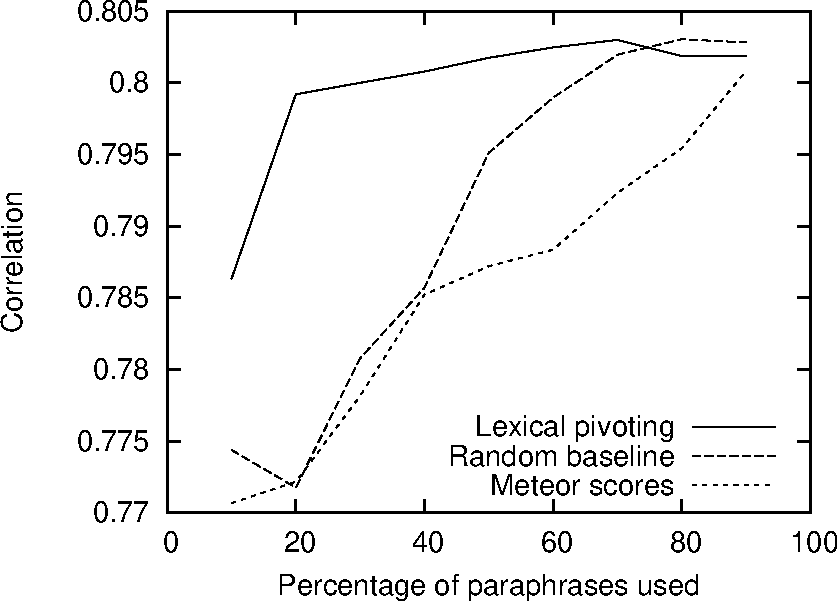
\includegraphics[scale=0.55]{../img/filtering-lexical-cropped.pdf}
\caption{Comparison of automatic filtering techniques for~\emph{one-word} paraphrases on WMT12 data.}
\label{fig:filtering-lexical}
\end{center}
\end{figure}

\begin{figure}[tb]
\begin{center}
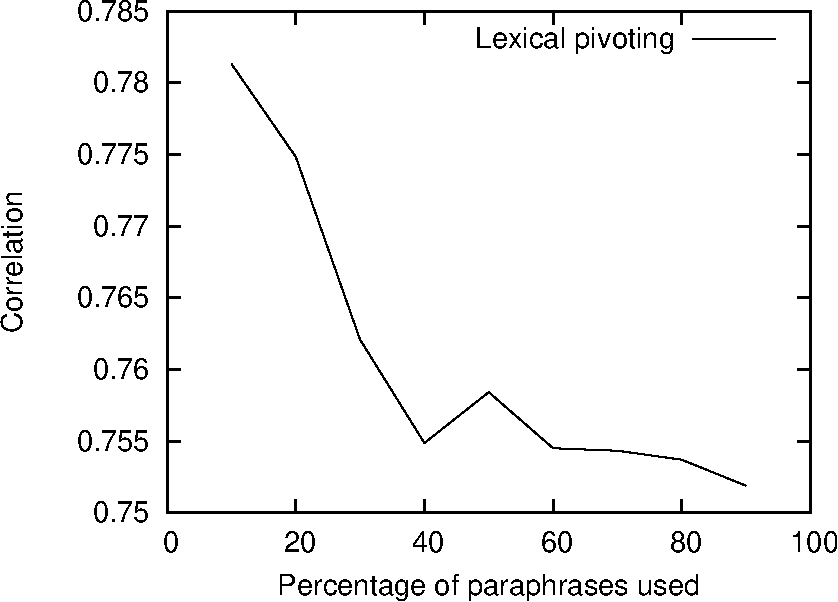
\includegraphics[scale=0.55]{../img/filtering-mwe-cropped.pdf}
\caption{Automatic filtering of multi-word paraphrase for~the \textit{multi-word-first} scenario on WMT12 data.}
\label{fig:filtering-mwe}
\end{center}
\end{figure}

\Fref{fig:filtering-lexical} shows the performance of different filtering
techniques for one-word paraphrases. Relying on the Meteor scores proves worse than
random selection. Using lexical pivoting, we can keep a high correlation even 
if we throw away as much as 80\% of the paraphrases, however we do not improve
(by~a~relevant margin) upon the baseline correlation of 0.802 achieved by
\emph{one-word-only} paraphrasing with the full paraphrase table.

We evaluate the best-performing technique also in the \textit{multi-word-first}
scenario where we use it for filtering multi-word paraphrases (see
\Fref{fig:filtering-mwe}). As we reduce the number of paraphrases, we observe a
considerable improvement of~correlation, however we never outperform
\textit{one-word-only} or \textit{one-word-first}. In this case, the filtering
simply mitigates the damage done by the multi-word paraphrases. We
cannot hope to achieve a higher score without a~more fine-grained grip on what
a~good multi-word paraphrase is.

\section{Results}
\label{results}

\begin{table*}[tb]
\begin{center}
\scalebox{0.99}{
\begin{tabular}{l|ccc|ccc}
\multicolumn{7}{c}{\textbf{WMT12}}\\
\hline
Method & \multicolumn{3}{c|}{Greedy selection} & \multicolumn{3}{c}{Word alignment} \\
\hline
Depfix & No  & Full  & Limited & No  & Full  & Limited\\
\hline
One-word only     & 0.80 & \textbf{0.83} & \textbf{0.83} & 0.79 & 0.81 & 0.81 \\
One-word first    & 0.79 & 0.82 & 0.82 & 0.77 & 0.79 & 0.80 \\
Multi-word first & 0.77 & 0.81 & 0.80 & 0.76 & 0.78 & 0.78 \\
\end{tabular}}
\vspace{10pt}
Baseline~correlation: \textbf{0.75}
\vspace{10pt}

\scalebox{0.99}{
\begin{tabular}{l|ccc|ccc}
\multicolumn{7}{c}{\textbf{WMT13}}\\
\hline
Method & \multicolumn{3}{c|}{Greedy selection} & \multicolumn{3}{c}{Word alignment} \\
\hline
Depfix & No  & Full  & Limited & No  & Full  & Limited\\
\hline
One-word only   & 0.86 & \textbf{0.89} & 0.88 & 0.86 & 0.88 & 0.87 \\
One-word first   & 0.85 & 0.88 & 0.88 & 0.83 & 0.87 & 0.86 \\
Multi-word first  & 0.84 & 0.87 & 0.86 & 0.83 & 0.87 & 0.86 \\
\end{tabular}}
Baseline~correlation: \textbf{0.83}

\caption{Pearson's correlation of BLEU and the silver standard.}
\label{corrs:12:13}
\end{center}
\end{table*}


The results of our algorithms are presented in \Tref{corrs:12:13}. The~baseline 
(i.e., using the original reference sentences) has a correlation of 0.75 and 0.83,
respectively. All evaluated approaches outperform it, the simplest one 
\textit{One-word only} performs the best. \Fref{example} shows an example of 
the \textit{One-word only} algorithm.

\begin{figure}[t]

\begin{center}
\begin{tabular}{ll}
 Source &  \begin{tabular}{l}
  	\textit{The location alone is classic.} \\
	\end{tabular} \\
 \hline
 
 Hypothesis & \begin{tabular}{llll}
 			\textit{Samotné} & \textit{místo} & \textit{je} & \textit{klasické.} \\
 			Actual & place & is & classic \\
			\end{tabular} \\
 &  \begin{tabular}{l}
  	The place alone is classic. \\
	\end{tabular} \\

 \hline
 Reference & \begin{tabular}{llll}
 			\textit{Už} & \textit{poloha} & \textit{je} & \textit{klasická.} \\
 			Already & position & is & classic. \\
			\end{tabular} \\
 &  \begin{tabular}{l}
  	The position itself is classic. \\
	\end{tabular}  \\ 

 \hline
  New reference & \begin{tabular}{llll}
 			\textit{Už} & \textit{místo} & \textit{je} & \textit{klasická.} \\
 			Already & place & is & classic \\
			\end{tabular} \\
 &  \begin{tabular}{l}
  	*The place itself is classic. \\
	\end{tabular} \\
 \hline 
  Depfixed ref. & \begin{tabular}{llll}
 			\textit{Už} & \textit{místo} & \textit{je} & \textit{klasické.} \\
 			Already & place & is & classic \\
			\end{tabular} \\
 &  \begin{tabular}{l}
  	The place itself is classic. \\
	\end{tabular} \\
 \hline  
 
\end{tabular}
\caption{Example of the \textit{One-word only} method. 
The~hypothesis is grammatically correct and has very similar meaning as the 
reference sentence. The new reference is closer in wording to the hypothesis, 
but there is grammatical disagreement between the noun and adjective. Depfix 
resolves the error and the final reference is correct and much more similar 
to~the hypothesis.}
\label{example}
\end{center}
\end{figure}

We use a test for comparing correlated correlation coefficients 
\citep{meng1992comparing} to determine whether the difference in correlation
coefficients is statistically significant. The test shows that BLEU performs
better with our reference sentences with 99\% certainty. 

Multi-word paraphrases are very noisy and while they do bring the system 
outputs closer to the reference (the average BLEU score of the systems 
increases), they often propose non-equivalent translations or violate the 
correctness of the sentence, thus blurring the differences between systems.
\todo{podlozit}

When paraphrasing is restricted by word alignment, all methods perform worse. 
As \Tref{substitutions:12:13} shows, the number of applied paraphrases is much
lower: while the proportion of correct paraphrases is higher, their amount is 
reduced too much and overall, our technique is harmed by this restriction. 
\todo{i tu chce marketa nejak dolozit, ze ta proporce spravnych parafrazi je vyssi}

\begin{table*}[htb]
\begin{center}
\begin{tabular}{l|cc|cc}
\multicolumn{5}{c}{\textbf{WMT12}}\\
\hline
\multirow{2}{*}{Method} & \multicolumn{2}{c|}{Greedy selection} & \multicolumn{2}{c}{Word alignment} \\
& Words & Phrases & Words & Phrases \\
\hline
One-word only     & 1.59 & --   & 0.86 &  --  \\
One-word first    & 1.59 & 0.23 & 0.86 & 0.22 \\
Multi-word first  & 1.38 & 0.31 & 0.81 & 0.27 \\
\end{tabular}
\vspace{10pt}
\begin{tabular}{l|cc|cc}
\multicolumn{5}{c}{\textbf{WMT13}}\\
\hline
\multirow{2}{*}{Method} & \multicolumn{2}{c|}{Greedy selection} & \multicolumn{2}{c}{Word alignment} \\
& Words & Phrases & Words & Phrases \\
\hline
One-word only    & 1.33 &  --  & 0.76 & --   \\
One-word first   & 1.33 & 0.20 & 0.76 & 0.20 \\
Multi-word first & 1.04 & 0.68 & 0.74 & 0.24 \\
\end{tabular}

\caption{Average number of replaced words/phrases per~sentence for each method 
on data from WMT12 and WMT13.}
\label{substitutions:12:13}
\end{center}
\end{table*}

On the other hand, applying Depfix is always beneficial, which supports our
 assumption of the importance of grammatical correctness of the created
references. However, the \textit{limited} version generally shows no 
improvement over the \textit{full} version.

Results on the data from WMT12 and WMT13 are consistent. Paraphrasing increases 
the accuracy of the evaluation using the BLEU metric, even though the 
differences in~the WMT13 data are not as~prominent due to a much higher 
baseline. This is also reflected in~the smaller amount of substitutions (see 
\Tref{substitutions:12:13}).

\section{Conclusion}
%Big difference in meteor (mozna zkusit jeste nejakou statistiku, jak casto dochazelo
%k substituci z meteoru a jak casto dochazi k substituci z meteoru x wordnetu? aby bylo
%opravdu mozne, ze ta filtrace vyznamne prispela??
Our results confirm the positive impact of paraphrasing a~reference sentence 
on~the performance of~the BLEU score. We~evaluate several approaches 
to~paraphrasing. The \textit{one-word only} greedy substitution method achieves 
the best results. We gain a statistically significant improvement in the 
evaluation of English-to-Czech MT. 

We illustrate several methods for reducing noise in a paraphrase corpus and
we confirm importance of grammar correctness of reference sentences in MT 
evaluation by the improvement of correlation after applying the Depfix system. 
\todo{odvazne tvrzeni, kdyz vime, ze tam Depfix i chyby zanasi - preformulovat}

%In the future, we plan to further increase the correlation by creating our own 
%Czech paraphrase tables that would be larger than Czech WordNet, but less noisy 
%than Czech Meteor Tables.

%Another way to improve the performance of our system which we want to follow
%is a further adaptation of the Depfix system to our task. We intend to
%tune existing Depfix corrections, as well as to add new corrections specific
%to our task. We would also like to devise a way of~informing Depfix which parts
%of the sentences come from the reference and which come from the paraphrasing
%to eliminate \equo{false positives}, i.e. Depfix attempting to correct words
%that are unlikely to be incorrect.

\chapter*{Conclusion}
\addcontentsline{toc}{chapter}{Conclusion}


%%% Bibliography
%%% Bibliography (literature used as a source)
%%%
%%% We employ bibTeX to construct the bibliography. It processes
%%% citations in the text (e.g., the \cite{...} macro) and looks up
%%% relevant entries in the bibliography.bib file.
%%%
%%% The \bibliographystyle command selects, which style will be used
%%% for references from the text. The argument in curly brackets is
%%% the name of the corresponding style file (*.bst). Both styles
%%% mentioned in this template are included in LaTeX distributions.

\bibliographystyle{plainnat}    %% Author (year)
% \bibliographystyle{unsrt}     %% [number]

\renewcommand{\bibname}{Bibliography}

%%% Generate the bibliography. Beware that if you cited no works,
%%% the empty list will be omitted completely.

\bibliography{bibliography}

%%% If case you prefer to write the bibliography manually (without bibTeX),
%%% you can use the following. Please follow the ISO 690 standard and
%%% citation conventions of your field of research.

% \begin{thebibliography}{99}
%
% \bibitem{lamport94}
%   {\sc Lamport,} Leslie.
%   \emph{\LaTeX: A Document Preparation System}.
%   2nd edition.
%   Massachusetts: Addison Wesley, 1994.
%   ISBN 0-201-52983-1.
%
% \end{thebibliography}


%%% Figures used in the thesis (consider if this is needed)
\listoffigures

%%% Tables used in the thesis (consider if this is needed)
%%% In mathematical theses, it could be better to move the list of tables to the beginning of the thesis.
\listoftables

%%% Abbreviations used in the thesis, if any, including their explanation
%%% In mathematical theses, it could be better to move the list of abbreviations to the beginning of the thesis.
\chapwithtoc{List of Abbreviations}
MRPC - Microsoft Research Paraphrase Corpus \\
MT - Machine Translation \\
WMT - Workshop on Statistical Machine Translation \\

%%% Doctoral theses must contain a list of author's publications
\chapwithtoc{List of publications}

%%% Attachments to the doctoral thesis, if any. Each attachment must be
%%% referred to at least once from the text of the thesis. Attachments
%%% are numbered.
%%%
%%% The printed version should preferably contain attachments, which can be
%%% read (additional tables and charts, supplementary text, examples of
%%% program output, etc.). The electronic version is more suited for attachments
%%% which will likely be used in an electronic form rather than read (program
%%% source code, data files, interactive charts, etc.). Electronic attachments
%%% should be uploaded to SIS and optionally also included in the thesis on a~CD/DVD.
%%% Allowed file formats are specified in provision of the rector no. 72/2017.
\appendix
\chapter{Attachments}

\section{First Attachment}

\openright
\end{document}
